\documentclass{article}

\usepackage{graphicx}
\usepackage{indentfirst}
\usepackage[a4paper, total={6in, 8in}]{geometry}
\usepackage{hyperref}
\usepackage{fancyhdr}
\usepackage{xepersian}
\settextfont{[XB Zar.ttf]}
\setlatintextfont{[Times New Roman.ttf]}

\begin{document}


%title page%
\begin{titlepage}
	\begin{center}
		\vspace{0.2cm}
		
		
\includegraphics[width=0.4\textwidth]{sharif.png}\\
		\vspace{0.2cm}
		\textbf{ \Huge{آزمایش شماره 10}}\\
		\vspace{0.25cm}
		\textbf{ \Large{آز شبکه - دکتر بردیا صفایی}}
		\vspace{0.2cm}
		
		
		\large \textbf{دانشکده مهندسی کامپیوتر}\\\vspace{0.1cm}
		\large   دانشگاه صنعتی شریف\\\vspace{0.2cm}
		\large   ﻧﯿﻢ‌سال اول ۰۱-۰۲ \\\vspace{0.10cm}
		\large{ گروه 8:}\\
		\large{\href{mailto:mehrshad.mirmohammadi@gmail.com}{مهرشاد میرمحمدی - 98109634}}\\
		\large{\href{mailto:parhaamsaremi@gmail.com}{پرهام صارمی - 97101959}}\\
		\large{\href{mailto:mofayezi.m@gmail.com}{محمدرضا مفیضی - 98106059}}\\
	\end{center}
\end{titlepage}
%title page%

\newpage

%pages header
\pagestyle{fancy}
\fancyhf{}
\fancyfoot{}
\setlength{\headheight}{59pt}
\cfoot{\thepage}
\lhead{آزمایش شماره 10}
\rhead{
\includegraphics[width=0.1\textwidth]{sharif.png}\\
		دانشکده مهندسی کامپیوتر
}
\chead{آز شبکه - گروه ۱۰}
%pages header


ابتدا در محیط \lr{packet tracer} سناریو گفته شده در کلاس را طراحی می‌کنیم (شکل \ref{fig:scenario-1}).
همانطور که از شکل \ref{fig:scenario-2} مشخص است، در ابتدا فقط VLAN شماره‌ی ۱ را داریم و لذا زمانی که یک آدرس را ping کنیم، سوییچ به همه‌ پیام می‌فرستد (شکل شماره‌ی \ref{fig:scenario-3}).

\begin{figure}[h!]
	\centering
	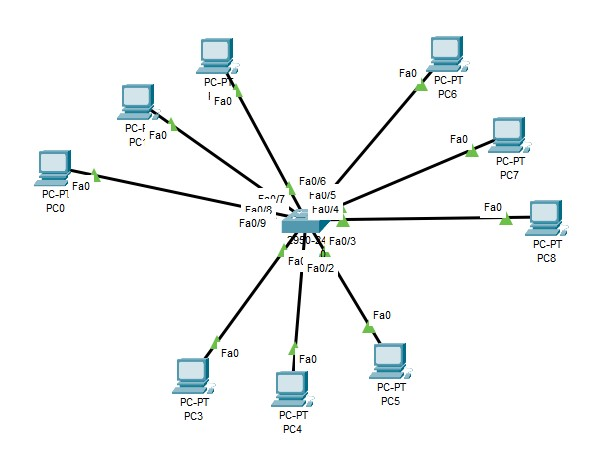
\includegraphics[width=0.6\columnwidth]{1.jpg}
	\caption{تصویر پیاده‌سازی سناریو در محیط \lr{packet tracer}}
	\label{fig:scenario-1}
\end{figure}

\begin{figure}[h!]
	\centering
	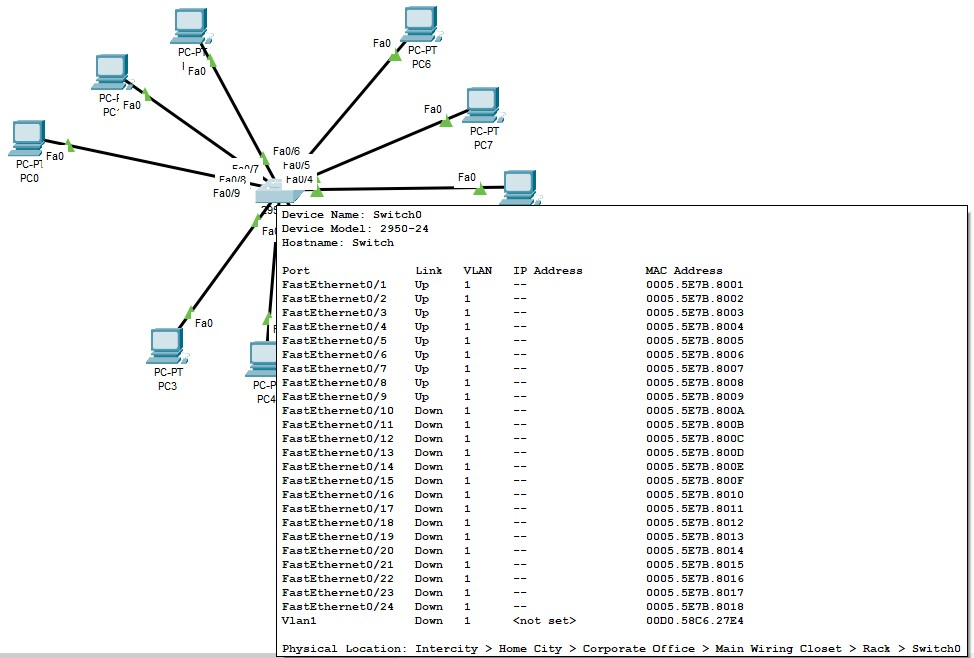
\includegraphics[width=0.6\columnwidth]{3.jpg}
	\caption{در ابتدا تنها VLAN شماره‌ی ۱ را داریم.}
	\label{fig:scenario-2}
\end{figure}

\begin{figure}[h!]
	\centering
	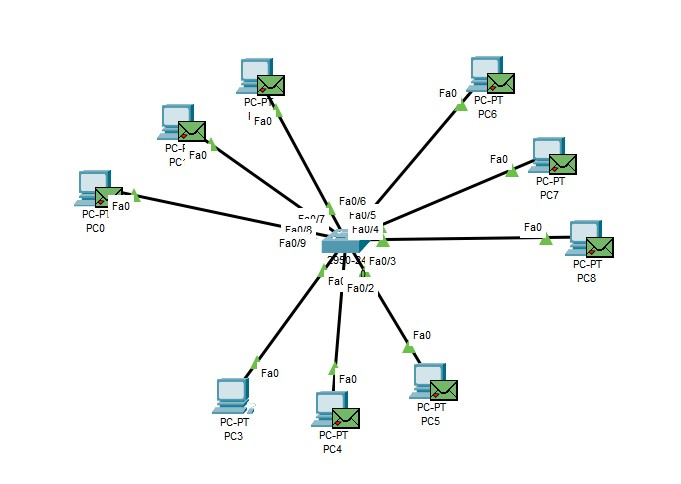
\includegraphics[width=0.6\columnwidth]{2.jpg}
	\caption{سوییچ به همه‌ی PC ها پیام می‌فرستد. این باعث هدر‌رفت يهنای باند می‌شود.}
	\label{fig:scenario-3}
\end{figure}

سپس برای تشکیل VLAN ها به CLI در سوییچ می‌رویم. دو VLAN  با شماره‌‌های ۲ و ۳ ایجاد می‌کنیم و به ترتیب به آنها نام‌های b و c را می‌دهیم. سپس interface‌ های شماره‌ی ۴ تا ۶ را به VLAN شماره‌ی ۲ و ۷ تا ۹ را به VLAN شماره‌ی ۳ وصل می‌کنیم (شکل‌های شماره‌ی \ref{fig:scenario-4} و \ref{fig:scenario-5}).

\begin{figure}[h!]
	\centering
	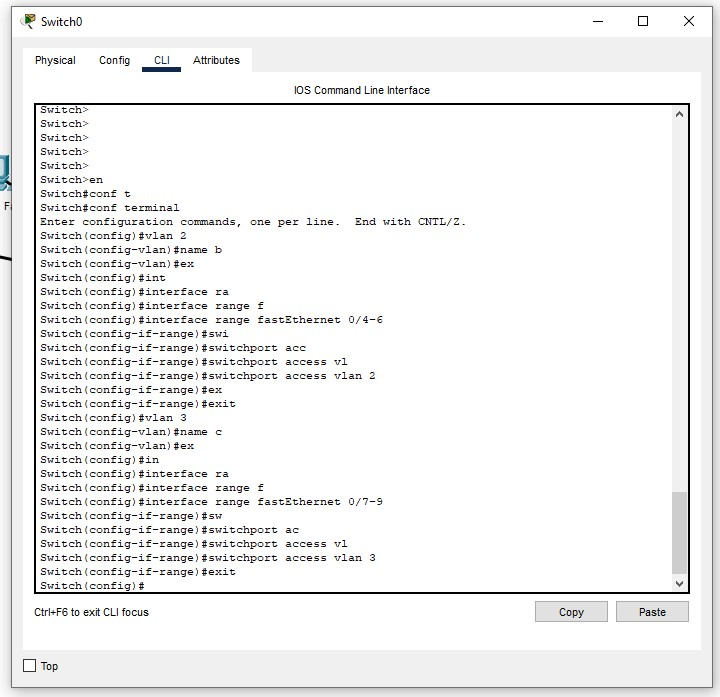
\includegraphics[width=0.6\columnwidth]{4.jpg}
	\caption{ساخت VLANهای جدید و وصل کردن interfaceها به آنها.}
	\label{fig:scenario-4}
\end{figure}

\begin{figure}[h!]
	\centering
	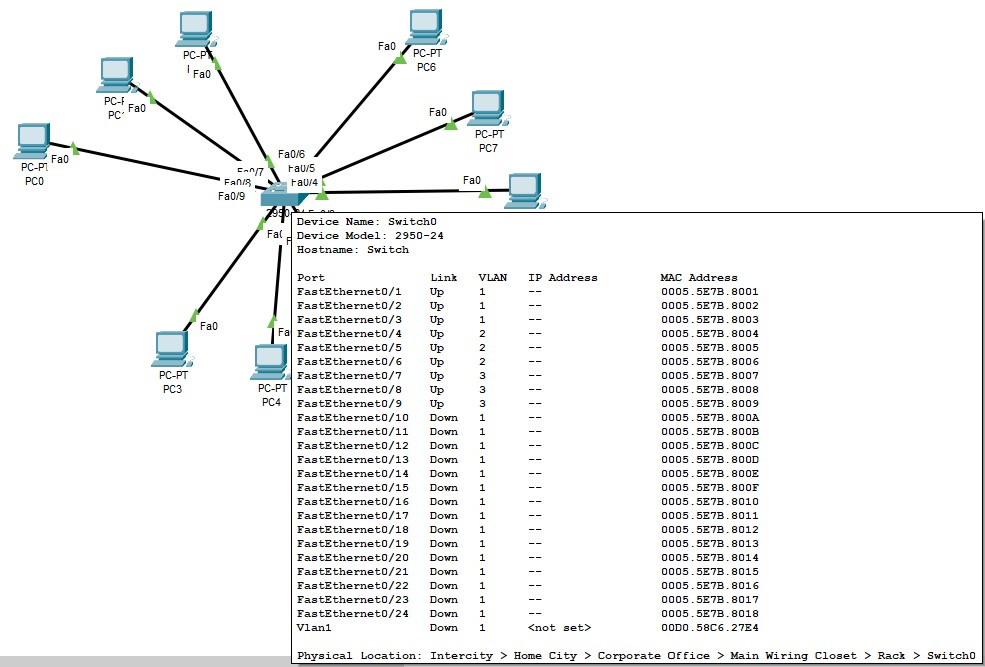
\includegraphics[width=0.6\columnwidth]{7.jpg}
	\caption{تناظر بین interface ها و VLAN ها}
	\label{fig:scenario-5}
\end{figure}

اکنون اگر از PC شماره‌ی ۳ آدرسی را ping کنیم، سوییچ فقط به دستگاه‌های داخل آن VLAN پیام می‌فرستد. برای PC شماره‌ی ۶ هم همین اتفاق می‌افتد (شکل‌‌های شماره‌ی \ref{fig:scenario-6} و \ref{fig:scenario-7}).

\begin{figure}[h!]
	\centering
	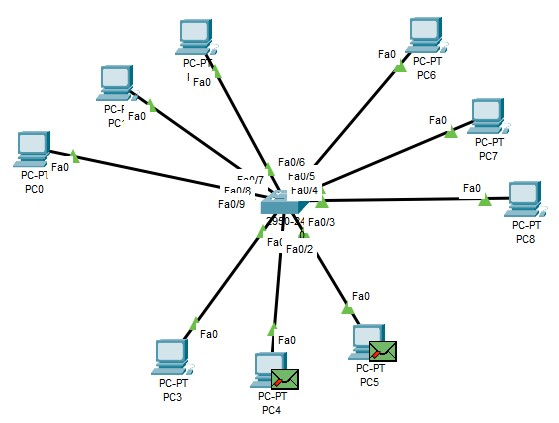
\includegraphics[width=0.6\columnwidth]{5.jpg}
	\caption{پیام‌های فرستاده شده از سمت سوییچ در زمان ping کردن توسط PC3}
	\label{fig:scenario-6}
\end{figure}

\begin{figure}[h!]
	\centering
	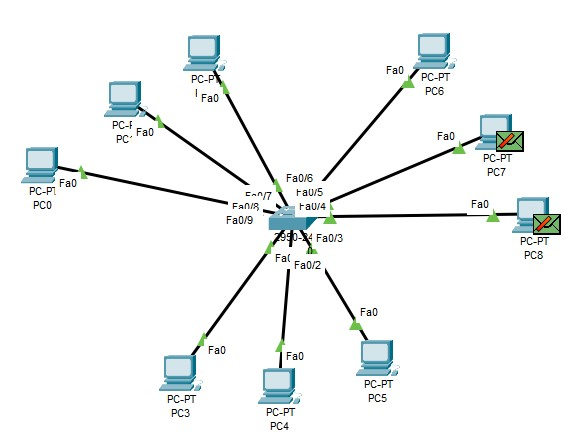
\includegraphics[width=0.6\columnwidth]{6.jpg}
	\caption{پیام‌های فرستاده شده از سمت سوییچ در زمان ping کردن توسط PC6}
	\label{fig:scenario-7}
\end{figure}

در نهایت با استفاده از دستور \textit{\lr{show vlan}} می‌توان دید کدام پورت‌ها به کدام VLAN ها متصل هستند و وضعیت هر کدام از VLAN ها چیست (شکل شکاره‌ی \ref{fig:scenario-8}).

\begin{figure}[h!]
	\centering
	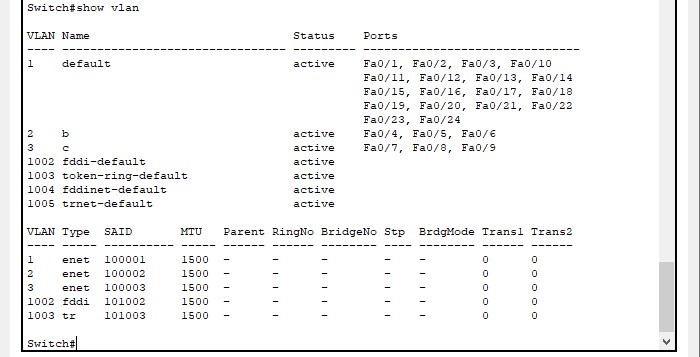
\includegraphics[width=0.6\columnwidth]{8.jpg}
	\caption{حاصل اجرای‌ دستور \textit{\lr{show vlan}} در داخل سوییچ}
	\label{fig:scenario-8}
\end{figure}

\end{document}
